% REPORT FOR PROJECT2 SF2565

\documentclass[a4paper,10pt]{article}

%%Packages	%%%	%%%	%%%	%%%	%%%	%%%	%%%
\usepackage{amsmath,framed}
\usepackage[latin1]{inputenc} 	
\usepackage{listings}
\usepackage{xcolor}
\usepackage{graphicx}
\usepackage{placeins}
\usepackage{textcomp}
%\usepackage{tikz}

%%Settings	%%%	%%%	%%%	%%%	%%%	%%%	%%%
\renewcommand{\d}{\text{d}}
\newcommand{\e}{\text{e}}
\newcommand{\ve}{\mathbf}
\newcommand\numb{\addtocounter{equation}{1}\tag{\theequation}}

\setlength\fboxsep{1.2mm}
\setlength\fboxrule{0.5mm}

\lstset { %
  language=C++,
  backgroundcolor=\color{black!3},	% set backgroundcolor
  basicstyle=\footnotesize,		% basic font setting
}

%%Margins	%%%	%%%	%%%	%%%	%%%	%%%	%%%
\usepackage{geometry}
\geometry{
  a4paper,
  left=35mm,
  right=35mm,
  top=35mm,
  bottom=35mm,
}

%%Header & Footer	%%%	%%%	%%%	%%%	%%%	%%%
\usepackage{fancyhdr}
\pagestyle{fancy}
\renewcommand{\headrulewidth}{1pt}
\rhead{Hanna Hultin, Mikael Perssson}
%8509080456 mitt persnr om vi vill ha det
\lhead{P4 SF565}

\title{Project 4, SF2565}
\author{Hanna Hultin, hhultin@kth.se, 931122-2468, TTMAM2 \\ Mikael Persson, mikaepe@kth.se, 850908-0456, TTMAM2}
\begin{document}
\maketitle

\subsection*{Task 1: Redesigning the Domain class}
The domain class was taken directly from project 3, with the following modifications. 
\begin{itemize}
  \item
    Functions \texttt{xsize()}, \texttt{ysize()} and \texttt{gridValid()} was added.
  \item The class uses \texttt{shared\_ptr} to the boundary curves. 
  \item
    The \texttt{writeFile()} function was changed to 
    \texttt{writeFile(std::string fileName)} to be able to save the 
    different grid functions with different filenames.
\end{itemize}
The \texttt{Curvebase} class and its derived classes are almost identical to those used in 
project 3. We have attempted to optimize the code slightly, for example by using inlining 
in the classes \texttt{xLine} and \texttt{yLine}.
\subsection*{Task 2: The Gfctn class}
The class for gridfunctions \texttt{class Gfctn} has the following data members.
\begin{itemize}
  \item
    A matrix \texttt{u} to store the grid function values.
  \item
    A \texttt{shared\_ptr} to a \texttt{Domain} object called \texttt{grid}.
\end{itemize}
The class has a the following constructors.
\begin{itemize}
  \item \texttt{Gfctn(shared\_ptr<Domain> grid)} which initializes the grid function with
    the matrix \texttt{u} being the zero matrix.
  \item \texttt{Gfctn(const Gfctn\& U)}, a copy constructor.
\end{itemize}
Overloaded operators are provided for adding and multiplying grid functions (\texttt{+} and 
\texttt{*}).
The following member functions are implemented.
\begin{itemize}
  \item
    \texttt{void setFunction(fctnPtr f)} which sets the gridfunction values to those
    defined by the function \texttt{f}. This function needs to take \texttt{Point}
    objects as argument.
  \item
    \texttt{void print()} which prints the matrix \texttt{u}.
    This is useful for testing on small grids only.
  \item
    \texttt{void writeFile(std::string fileName) const} which saves the grid function
    values to a binary file, \texttt{fileName.bin}.
\end{itemize}
In addition to those functions listed above, the class has functions to compute 
the approximations to $\tfrac{\partial u}{\partial x}$, $\tfrac{\partial u}{\partial y}$,
$\tfrac{\partial^2 u}{\partial x^2}$ and $\tfrac{\partial^2 u}{\partial y^2}$.
Finally the class has a function for computing the Laplacian of the grid function, 
$\Delta u = \tfrac{\partial^2 u}{\partial x^2} + \tfrac{\partial^2 u}{\partial y^2}$.
These functions are
\begin{itemize}
  \item
    \texttt{Gfctn D0x() const}
  \item
    \texttt{Gfctn D0y() const}
  \item
    \texttt{Gfctn DD0x() const}
  \item
    \texttt{Gfctn DD0y() const}
  \item
    \texttt{Gfctn laplace() const}
\end{itemize}
    




\subsection*{Task 3: Results}
We investigate the class using the function
\begin{equation*}
  u(x,y) = \sin (x^2/10^2) \cos (x/10) + y
\end{equation*}
Figure 1 shows the function on the domain from project 3.
\begin{figure}[ht!]
  \centering
  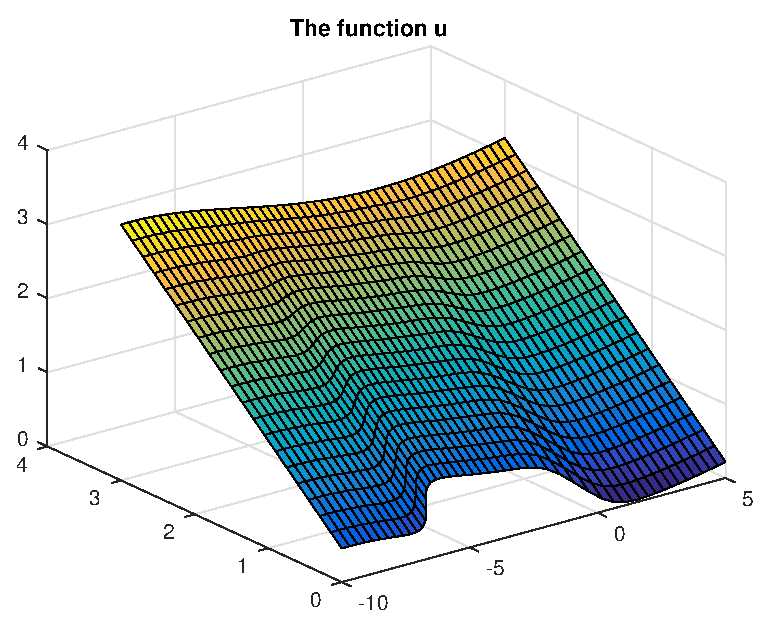
\includegraphics[width = 10cm, height = 8cm]{ufctn}
  \begin{minipage}[t]{100mm}
    \caption{
      TODO caption
    }\label{FIG_jjj}
  \end{minipage}
\end{figure}

\subsection*{Derivative w.r.t. $x$}

Figures 2 and 3 shows the derivative w.r.t. $x$ and the result from the implementation.
Figure 4 show the difference between the true derivative w.r.t $x$ and the implementation.



\begin{figure}[ht]
  \centering
  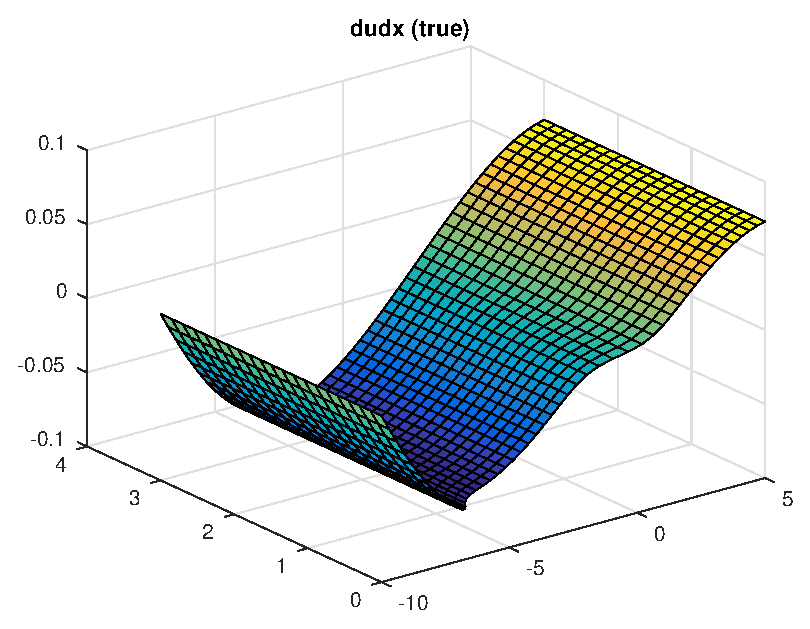
\includegraphics[width = 10cm, height = 8cm]{dudx}
  \begin{minipage}[t]{100mm}
    \caption{
      The true derivative $\tfrac{\partial u}{\partial x}$.
    }\label{FIG_jjj}
  \end{minipage}
\end{figure}


\begin{figure}[ht]
  \centering
  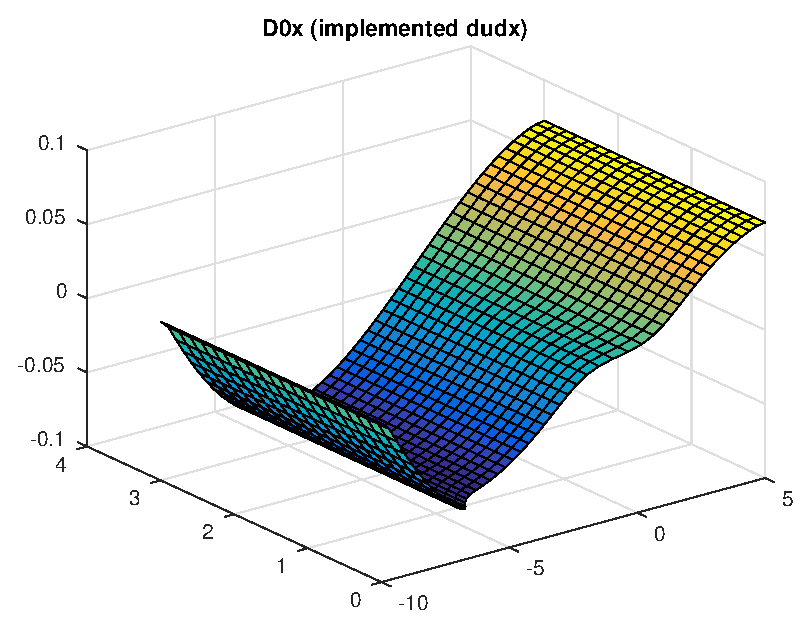
\includegraphics[width = 10cm, height = 8cm]{D0x}
  \begin{minipage}[t]{100mm}
    \caption{
      The result of the implementation of the derivative $\tfrac{\partial u}{\partial x}$.
    }\label{FIG_jjj}
  \end{minipage}
\end{figure}



\begin{figure}[ht]
  \centering
  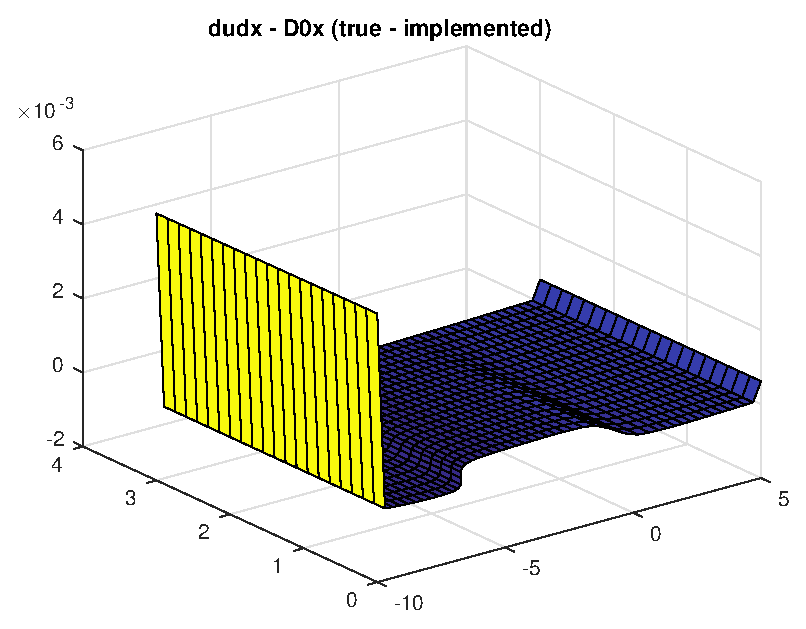
\includegraphics[width = 10cm, height = 8cm]{dudxD0x}
  \begin{minipage}[t]{100mm}
    \caption{
      The difference of the true and implemented $x$-derivatives. Since we used
      one-sided differences on the boundary, the accuracy of the implementation is
      lower at the boundary. 
    }\label{FIG_jjj}
  \end{minipage}
\end{figure}



\FloatBarrier
\subsection*{Derivative w.r.t. $y$}
Figure 5 shows the true derivative w.r.t. $y$ while figures 6 and 7 show the implemented derivative
and the difference of the true and implemented derivatives.
\FloatBarrier

\begin{figure}[ht]
  \centering
  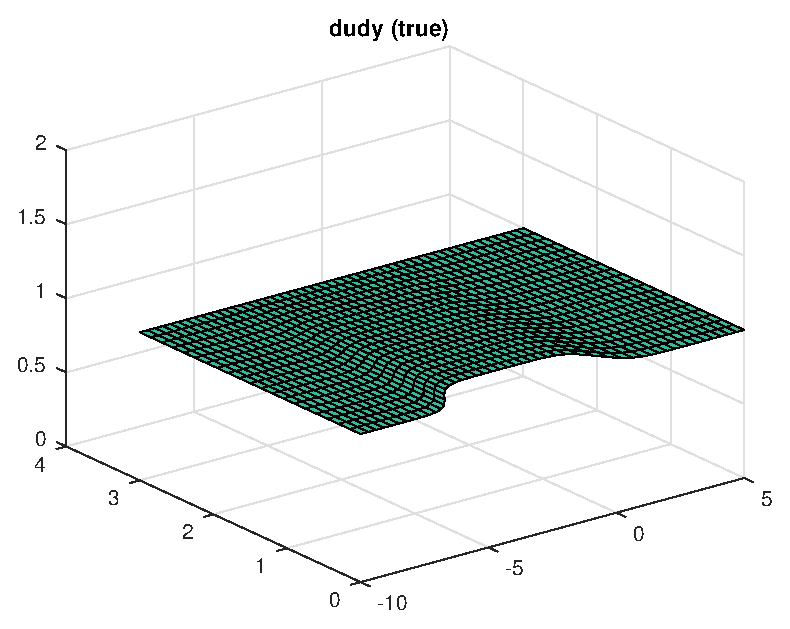
\includegraphics[width = 10cm, height = 8cm]{dudy}
  \begin{minipage}[t]{100mm}
    \caption{
      The true derivative $\tfrac{\partial u}{\partial y}$ is constant and
      equal to 1.
    }\label{FIG_jjj}
  \end{minipage}
\end{figure}


\begin{figure}[ht]
  \centering
  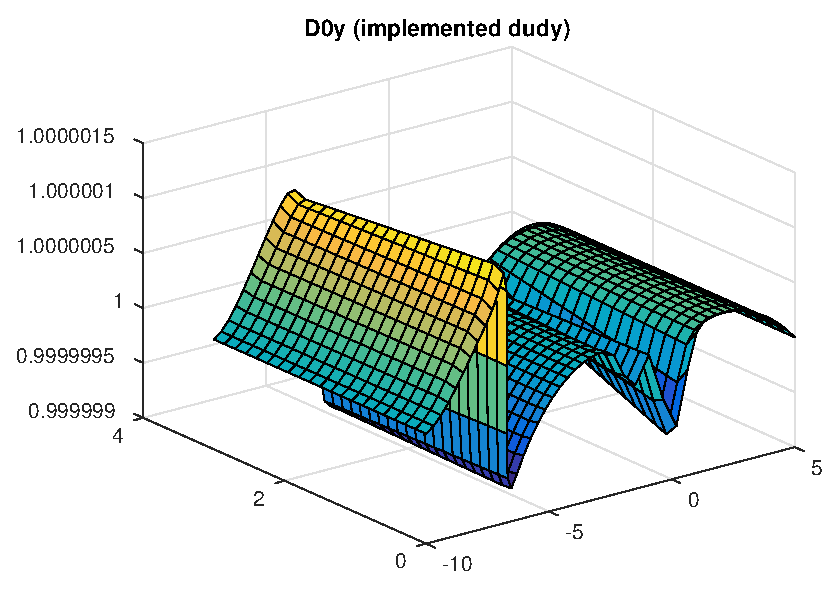
\includegraphics[width = 10cm, height = 8cm]{D0y}
  \begin{minipage}[t]{100mm}
    \caption{
      The implemented $y$-derivative. It is almost constantly equal to 1.
    }\label{FIG_jjj}
  \end{minipage}
\end{figure}



\begin{figure}[ht]
  \centering
  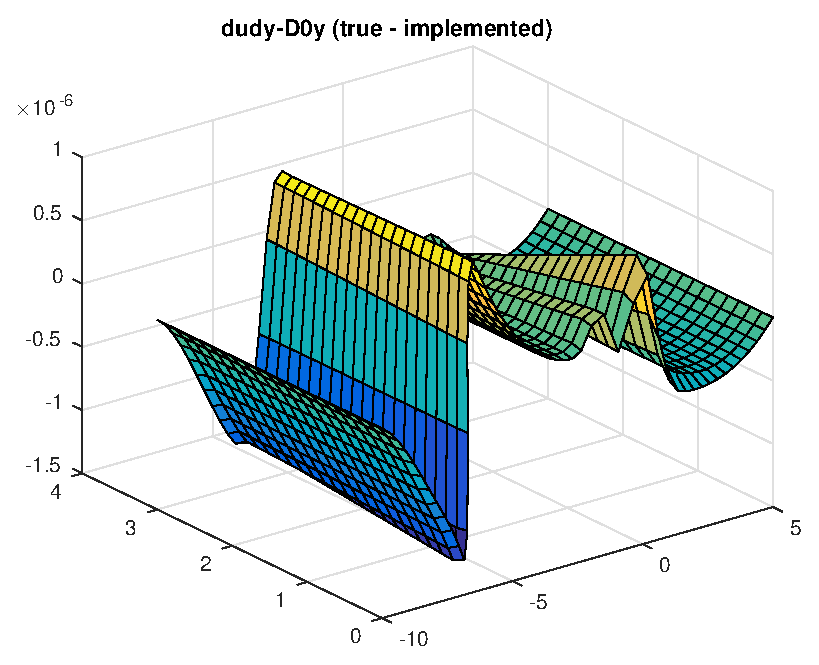
\includegraphics[width = 10cm, height = 8cm]{dudyD0y}
  \begin{minipage}[t]{100mm}
    \caption{
      Difference between true and implemented derivatives.
    }\label{FIG_jjj}
  \end{minipage}
\end{figure}

\FloatBarrier

\subsection*{Laplace operator}

\begin{figure}[ht]
  \centering
  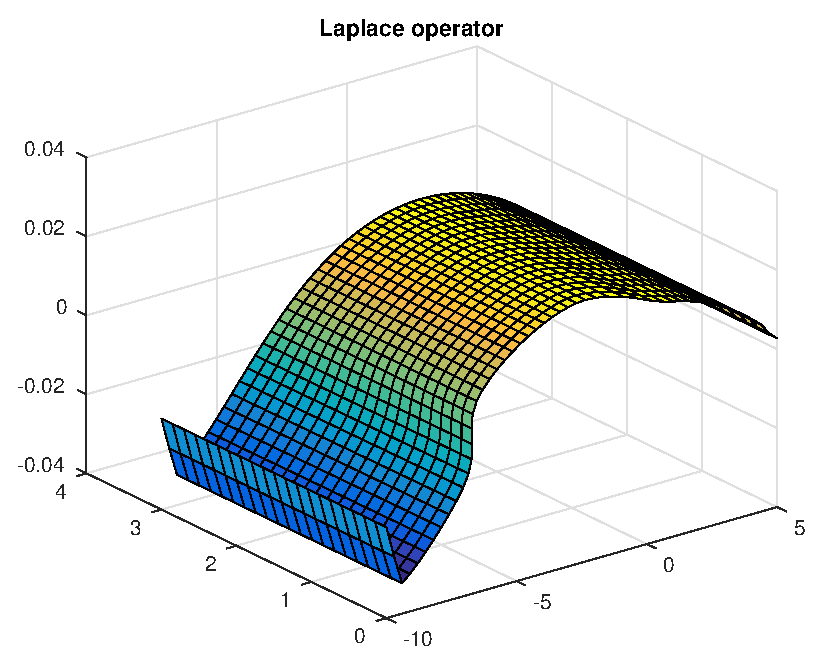
\includegraphics[width = 10cm, height = 8cm]{Laplace}
  \begin{minipage}[t]{100mm}
    \caption{
      The Laplacian of the grid function $u$.
    }\label{FIG_jjj}
  \end{minipage}
\end{figure}







\FloatBarrier
\newpage
\subsection*{Code}
\subsubsection*{Main}
\lstinputlisting[language=C++,basicstyle=\scriptsize]{../main1.cpp}
\subsubsection*{The Curvebase Class}
\lstinputlisting[language=C++,basicstyle=\scriptsize]{../curvebase.hpp}
\lstinputlisting[language=C++,basicstyle=\scriptsize]{../curvebase.cpp}
\subsubsection*{The derived classes from the Curvebase Class}
\texttt{yline}).
\lstinputlisting[language=C++,basicstyle=\scriptsize]{../xline.hpp}
%\lstinputlisting[language=C++,basicstyle=\scriptsize]{../xline.cpp}
\lstinputlisting[language=C++,basicstyle=\scriptsize]{../yline.hpp}
%\lstinputlisting[language=C++,basicstyle=\scriptsize]{../yline.cpp}
\lstinputlisting[language=C++,basicstyle=\scriptsize]{../fxcurve.hpp}
\lstinputlisting[language=C++,basicstyle=\scriptsize]{../fxcurve.cpp}
\subsubsection*{The Domain Class}
\lstinputlisting[language=C++,basicstyle=\scriptsize]{../domain.hpp}
\lstinputlisting[language=C++,basicstyle=\scriptsize]{../domain.cpp}

\subsubsection*{The Gfctn Class}
\lstinputlisting[language=C++,basicstyle=\scriptsize]{../gfctn.hpp}
\lstinputlisting[language=C++,basicstyle=\scriptsize]{../gfctn.cpp}

\subsubsection*{The Matrix Class}
\lstinputlisting[language=C++,basicstyle=\scriptsize]{../matrix.hpp}
\lstinputlisting[language=C++,basicstyle=\scriptsize]{../matrix.cpp}

\subsubsection*{The Point Class}
\lstinputlisting[language=C++,basicstyle=\scriptsize]{../point.hpp}
\lstinputlisting[language=C++,basicstyle=\scriptsize]{../point.cpp}



\end{document}





